\documentclass[10pt,a4paper,twocolumn]{article}

\usepackage[a4paper,margin=20mm]{geometry}

\usepackage[T1]{fontenc}\usepackage{lmodern}\input{glyphtounicode}\pdfgentounicode=1

\usepackage{amsmath,graphicx,fancyhdr,caption}

\pagestyle{fancy}\fancyhf{}\fancyhead[C]{\small\itshape Notes on Tidal Mixing - Draft}\fancyfoot[C]{\thepage}\renewcommand{\headrulewidth}{0pt}

\title{A Simple Model of Mixing in Shallow Estuaries}\author{Ada Rowntree\textsuperscript{1}, Tomas Elling\textsuperscript{2}\\ \small\textsuperscript{1}Coastal Laboratory, Port Amble. \textsuperscript{2}School of Water Studies, Hollin Vale.}\date{}

\begin{document}

\twocolumn[\maketitle\thispagestyle{fancy}\begin{center}\begin{minipage}{0.7\textwidth}\centerline{\bfseries Abstract}\smallskip\small We describe a two-box model of salt and fresh water in a shallow estuary. The model needs only the river flow, the tidal range and one mixing constant, and it reproduces the salinity measured at six stations within a few units. We fit the constant from one season of readings and test it on the next.\end{minipage}\end{center}\bigskip]

\section*{1 Introduction}

A shallow estuary mixes river water with sea water twice a day. Its salinity at a place depends on the river flow, on the tide and on how fast the two waters stir. Many models describe this with care; ours keeps only what a harbour office can measure. We call the salinity of box $i$ the value $s_i$ and the river flow $Q$, and we take the mixing to grow with the square of the tidal range, $r^2$.\footnote{The six stations are the ones used by the harbour survey of the same year.} The rest of this note sets out the model, fits it and tests it.

\begin{equation}\frac{ds}{dt} = k\,(s_0 - s)\tag{1}\end{equation}

Equation 1 says that each box relaxes toward the sea value at a rate set by the constant k. The constant is the only number we fit, and the next section shows how.

\section*{2 Method}

We read the salinity at six stations at high and low water for one season. For each station we took the mean of the two readings of a day and the river flow of the same day from the gauge above the town. The flux between two boxes is then written as a sum of the river term and the mixing term.

\begin{equation}F = Q\,s + k\,A\,r^2\tag{2}\end{equation}

Here $A$ is the cross-section of the channel at the boundary. We fitted $k$ by least squares over all days of the first season and kept the second season apart for the test.

\begin{figure*}[t]\centering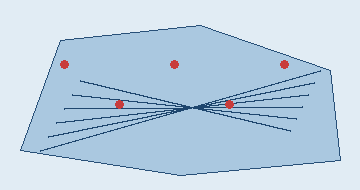
\includegraphics[width=0.6\textwidth]{figure.png}\caption*{Figure 1: Salinity along the channel at high water.}\end{figure*}

\begin{table*}[t]\centering\caption*{Table 1: Fitted constants for the two seasons.}\begin{tabular}{|l|c|c|}\hline \textbf{Season} & \textbf{k (per day)} & \textbf{Error} \\ \hline Spring & 0.42 & 1.8 \\ \hline Autumn & 0.39 & 2.1 \\ \hline Both & 0.41 & 1.9 \\ \hline\end{tabular}\end{table*}

\section*{3 Results}

The fitted constant changed little between the seasons, as Table 1 shows. The model followed the measured salinity at five of the six stations; at the sixth, close to the weir, it ran high on every spring tide.\footnote{Readings taken in storms were left out of the fit.} We think the weir holds back fresh water that the model lets through.

\section*{References}

\small

\par\noindent\hangindent=1.5em\hangafter=1 [1] Calloway, P. and Dene, M. Tides of small harbours. Coastal Notes 4, 2019, pages 11 to 29.

\par\noindent\hangindent=1.5em\hangafter=1 [2] Rowntree, A. Salinity readings at Port Amble, a working record kept for the harbour office over three seasons. Port Amble, 2024.

\par\noindent\hangindent=1.5em\hangafter=1 [3] Elling, T. Box models for teaching. Hollin Vale Press, 2021.

\end{document}